\documentclass[14pt]{extbook}
\usepackage{multicol, enumerate, enumitem, hyperref, color, soul, setspace, parskip, fancyhdr} %General Packages
\usepackage{amssymb, amsthm, amsmath, bbm, latexsym, units, mathtools} %Math Packages
\everymath{\displaystyle} %All math in Display Style
% Packages with additional options
\usepackage[headsep=0.5cm,headheight=12pt, left=1 in,right= 1 in,top= 1 in,bottom= 1 in]{geometry}
\usepackage[usenames,dvipsnames]{xcolor}
\usepackage{dashrule}  % Package to use the command below to create lines between items
\newcommand{\litem}[1]{\item#1\hspace*{-1cm}\rule{\textwidth}{0.4pt}}
\pagestyle{fancy}
\lhead{Progress Quiz 3}
\chead{}
\rhead{Version A}
\lfoot{}
\cfoot{}
\rfoot{Fall 2020}
\begin{document}

\begin{enumerate}
\litem{
Which of the following equations \textit{could} be of the graph presented below?
\begin{center}
    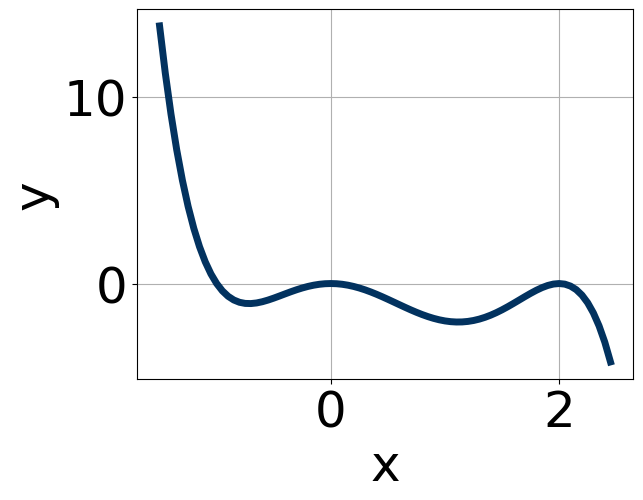
\includegraphics[width=0.5\textwidth]{../Figures/polyGraphToFunctionA.png}
\end{center}
\begin{enumerate}[label=\Alph*.]
\item \( -5(x + 4)^{4} (x - 1)^{4} (x - 3)^{6} \)
\item \( 7(x + 4)^{4} (x - 1)^{6} (x - 3)^{6} \)
\item \( 2(x + 4)^{6} (x - 1)^{10} (x - 3)^{7} \)
\item \( 6(x + 4)^{6} (x - 1)^{5} (x - 3)^{11} \)
\item \( -17(x + 4)^{10} (x - 1)^{10} (x - 3)^{11} \)

\end{enumerate} }
\litem{
Construct the lowest-degree polynomial given the zeros below. Then, choose the intervals that contain the coefficients of the polynomial in the form $x^3+bx^2+cx+d$.\[ 5 + 4 i \text{ and } 2 \]\begin{enumerate}[label=\Alph*.]
\item \( b \in [1, 8], c \in [-7.98, -6.69], \text{ and } d \in [9.7, 10.6] \)
\item \( b \in [1, 8], c \in [-6.23, -5.01], \text{ and } d \in [6.5, 9.7] \)
\item \( b \in [-15, -10], c \in [60.98, 61.96], \text{ and } d \in [-84.3, -79.9] \)
\item \( b \in [8, 15], c \in [60.98, 61.96], \text{ and } d \in [80.1, 83.9] \)
\item \( \text{None of the above.} \)

\end{enumerate} }
\litem{
Construct the lowest-degree polynomial given the zeros below. Then, choose the intervals that contain the coefficients of the polynomial in the form $ax^3+bx^2+cx+d$.\[ \frac{-2}{3}, \frac{4}{5}, \text{ and } \frac{-1}{4} \]\begin{enumerate}[label=\Alph*.]
\item \( a \in [58, 61], b \in [-8, -6], c \in [-40, -31], \text{ and } d \in [1, 11] \)
\item \( a \in [58, 61], b \in [14, 25], c \in [-31, -29], \text{ and } d \in [-10, -6] \)
\item \( a \in [58, 61], b \in [-73, -63], c \in [5, 13], \text{ and } d \in [1, 11] \)
\item \( a \in [58, 61], b \in [-4, 10], c \in [-40, -31], \text{ and } d \in [-10, -6] \)
\item \( a \in [58, 61], b \in [-4, 10], c \in [-40, -31], \text{ and } d \in [1, 11] \)

\end{enumerate} }
\litem{
Which of the following equations \textit{could} be of the graph presented below?
\begin{center}
    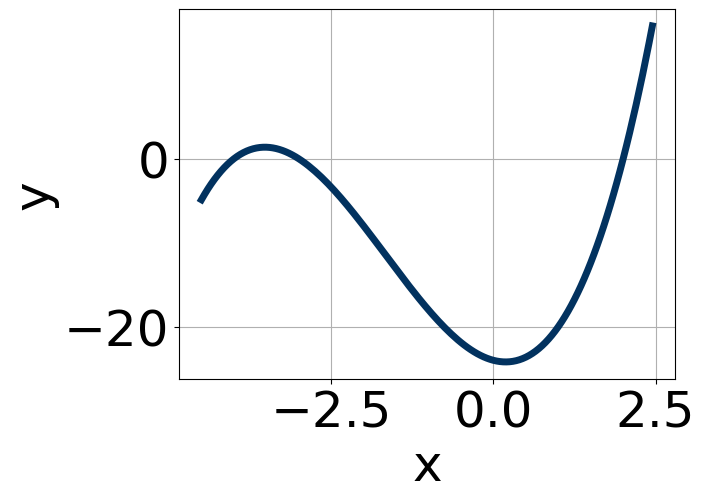
\includegraphics[width=0.5\textwidth]{../Figures/polyGraphToFunctionCopyA.png}
\end{center}
\begin{enumerate}[label=\Alph*.]
\item \( 16(x + 3)^{5} (x - 2)^{11} (x + 4)^{7} \)
\item \( 4(x + 3)^{8} (x - 2)^{10} (x + 4)^{11} \)
\item \( -16(x + 3)^{11} (x - 2)^{5} (x + 4)^{5} \)
\item \( -20(x + 3)^{6} (x - 2)^{5} (x + 4)^{11} \)
\item \( 20(x + 3)^{6} (x - 2)^{7} (x + 4)^{7} \)

\end{enumerate} }
\litem{
Construct the lowest-degree polynomial given the zeros below. Then, choose the intervals that contain the coefficients of the polynomial in the form $ax^3+bx^2+cx+d$.\[ \frac{3}{2}, \frac{2}{5}, \text{ and } \frac{3}{4} \]\begin{enumerate}[label=\Alph*.]
\item \( a \in [38, 49], b \in [38, 47], c \in [-40, -29], \text{ and } d \in [-23, -17] \)
\item \( a \in [38, 49], b \in [13, 17], c \in [-58, -53], \text{ and } d \in [13, 20] \)
\item \( a \in [38, 49], b \in [-108, -98], c \in [72, 89], \text{ and } d \in [-23, -17] \)
\item \( a \in [38, 49], b \in [-108, -98], c \in [72, 89], \text{ and } d \in [13, 20] \)
\item \( a \in [38, 49], b \in [103, 112], c \in [72, 89], \text{ and } d \in [13, 20] \)

\end{enumerate} }
\litem{
Describe the end behavior of the polynomial below.\[ f(x) = 2(x + 6)^{5}(x - 6)^{8}(x - 4)^{3}(x + 4)^{3} \]\begin{enumerate}[label=\Alph*.]
\begin{multicols}{2}\item 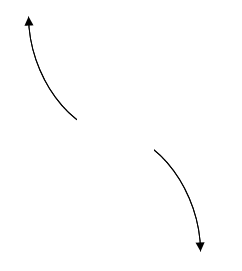
\includegraphics[width = 0.3\textwidth]{../Figures/polyEndBehaviorAA.png}\item 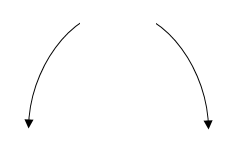
\includegraphics[width = 0.3\textwidth]{../Figures/polyEndBehaviorBA.png}\item 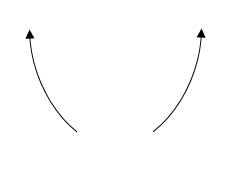
\includegraphics[width = 0.3\textwidth]{../Figures/polyEndBehaviorCA.png}\item 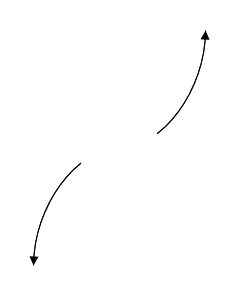
\includegraphics[width = 0.3\textwidth]{../Figures/polyEndBehaviorDA.png}\end{multicols}\item None of the above.
\end{enumerate} }
\litem{
Describe the zero behavior of the zero $x = -7$ of the polynomial below.\[ f(x) = 3(x - 7)^{4}(x + 7)^{7}(x - 4)^{4}(x + 4)^{7} \]\begin{enumerate}[label=\Alph*.]
\begin{multicols}{2}\item 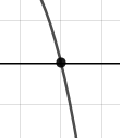
\includegraphics[width = 0.3\textwidth]{../Figures/polyZeroBehaviorAA.png}\item 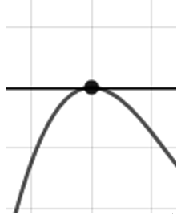
\includegraphics[width = 0.3\textwidth]{../Figures/polyZeroBehaviorBA.png}\item 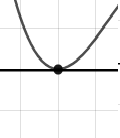
\includegraphics[width = 0.3\textwidth]{../Figures/polyZeroBehaviorCA.png}\item 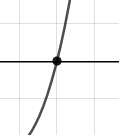
\includegraphics[width = 0.3\textwidth]{../Figures/polyZeroBehaviorDA.png}\end{multicols}\item None of the above.
\end{enumerate} }
\litem{
Describe the zero behavior of the zero $x = 3$ of the polynomial below.\[ f(x) = 5(x - 9)^{4}(x + 9)^{3}(x + 3)^{9}(x - 3)^{8} \]\begin{enumerate}[label=\Alph*.]
\begin{multicols}{2}\item 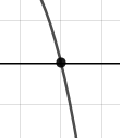
\includegraphics[width = 0.3\textwidth]{../Figures/polyZeroBehaviorCopyAA.png}\item 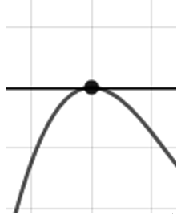
\includegraphics[width = 0.3\textwidth]{../Figures/polyZeroBehaviorCopyBA.png}\item 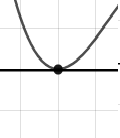
\includegraphics[width = 0.3\textwidth]{../Figures/polyZeroBehaviorCopyCA.png}\item 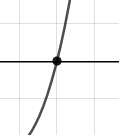
\includegraphics[width = 0.3\textwidth]{../Figures/polyZeroBehaviorCopyDA.png}\end{multicols}\item None of the above.
\end{enumerate} }
\litem{
Describe the end behavior of the polynomial below.\[ f(x) = -8(x + 9)^{2}(x - 9)^{3}(x - 4)^{2}(x + 4)^{2} \]\begin{enumerate}[label=\Alph*.]
\begin{multicols}{2}\item 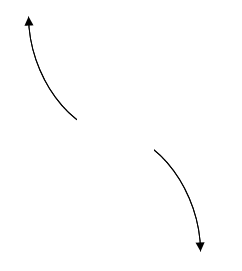
\includegraphics[width = 0.3\textwidth]{../Figures/polyEndBehaviorCopyAA.png}\item 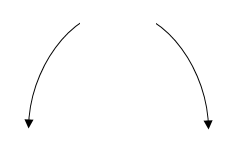
\includegraphics[width = 0.3\textwidth]{../Figures/polyEndBehaviorCopyBA.png}\item 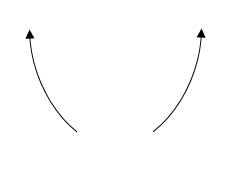
\includegraphics[width = 0.3\textwidth]{../Figures/polyEndBehaviorCopyCA.png}\item 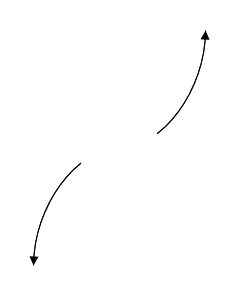
\includegraphics[width = 0.3\textwidth]{../Figures/polyEndBehaviorCopyDA.png}\end{multicols}\item None of the above.
\end{enumerate} }
\litem{
Construct the lowest-degree polynomial given the zeros below. Then, choose the intervals that contain the coefficients of the polynomial in the form $x^3+bx^2+cx+d$.\[ 3 - 3 i \text{ and } 1 \]\begin{enumerate}[label=\Alph*.]
\item \( b \in [-15, -5], c \in [18, 28], \text{ and } d \in [-19.7, -15.4] \)
\item \( b \in [1, 2], c \in [-6, -1], \text{ and } d \in [1.5, 3.1] \)
\item \( b \in [3, 8], c \in [18, 28], \text{ and } d \in [17.8, 20.6] \)
\item \( b \in [1, 2], c \in [-2, 7], \text{ and } d \in [-3.5, 0.4] \)
\item \( \text{None of the above.} \)

\end{enumerate} }
\end{enumerate}

\end{document}